\documentclass{beamer}
\usepackage[english,russian]{babel}
\usepackage[utf8]{inputenc}
\usepackage{amsmath}
\usepackage{hyperref}
\usetheme{Warsaw}
\usepackage{listings}
\usepackage{xcolor}
\usepackage{tikz}
\usetikzlibrary{graphs}
\usepackage{algpseudocode}

\lstset{
    frame=tb,
    tabsize=4,
    showstringspaces=false,
    numbers=left,
    commentstyle=\color{green},
    keywordstyle=\color{blue},
    stringstyle=\color{red},
    emph={baz},
    emphstyle=\textbf
}
\begin{document}

\title{Задачи разрешимости логических формул и приложения\newline Лекция 10. Комбинирование логик}
\author{Роман Холин}
\institute{Московский государственный университет}
\date{Москва, 2021}

\begin{frame}
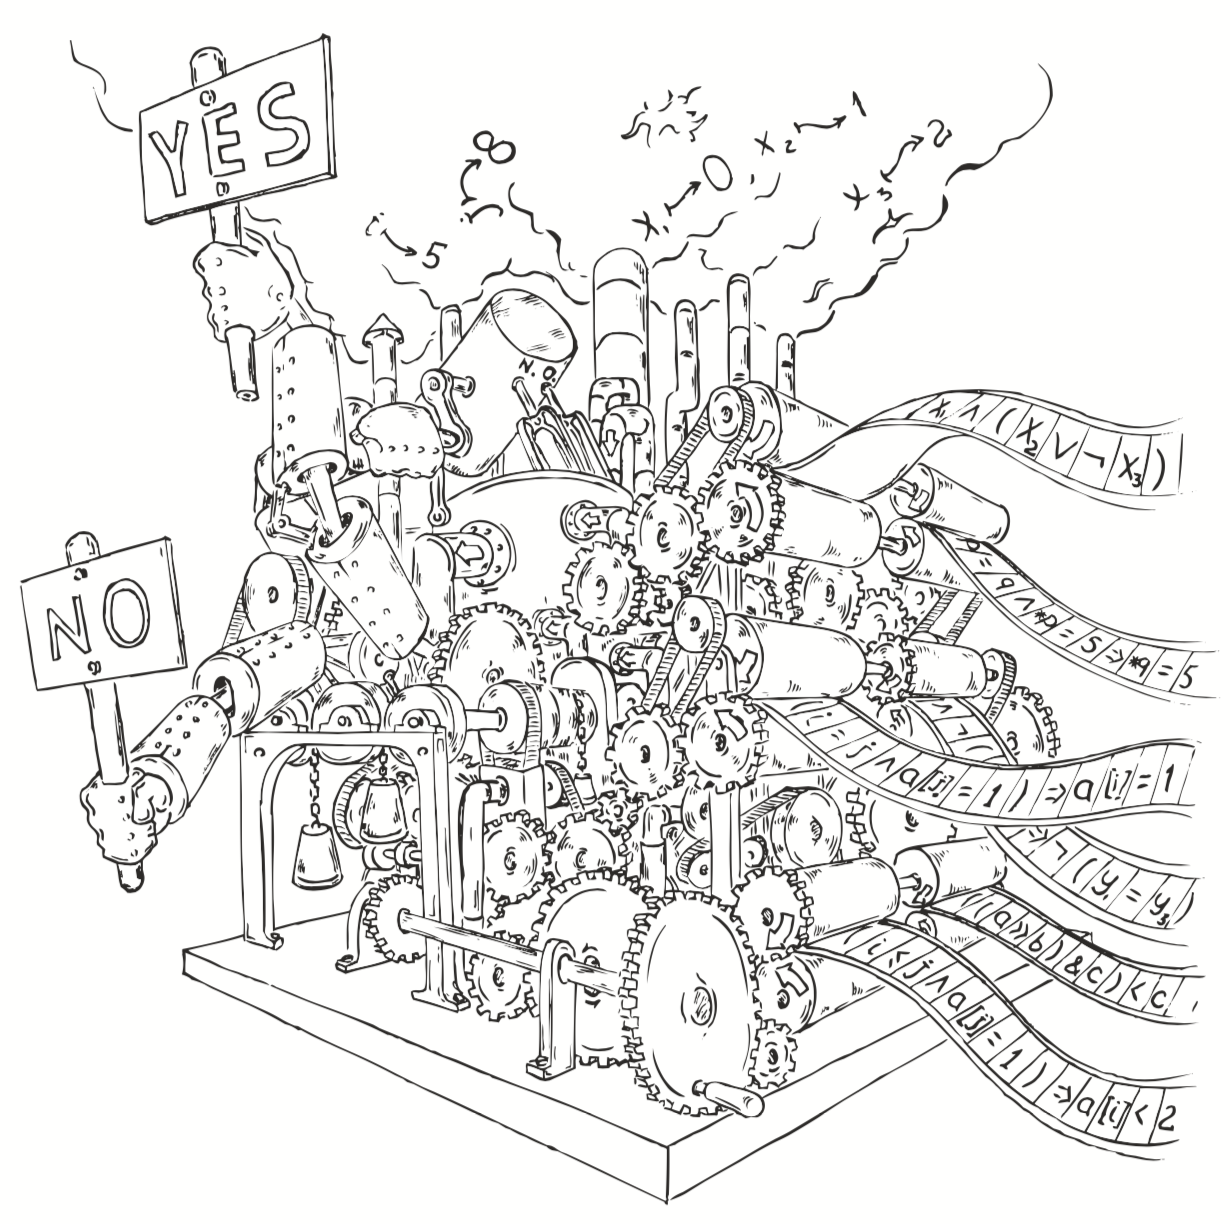
\includegraphics[scale=0.5]{../decision-procedure.png}
\end{frame}

\frame{\titlepage}

\begin{frame}{Зачему нужно комбинировать теории?}
\begin{enumerate}
\item Комбинации линейной арифметики и неинтрепретируемых функций:\newline
$(x_2 \ge x_1 ) \wedge (x_1 - x_3 \ge x 2 ) \wedge (x_3 \ge 0) \wedge f(f(x_1) - f(x_2)) \ne f(x_3)$
\item Комбинации битовых векторов и неинтрепретируемых функций:\newline
$f(a[32], b[1]) = f (b[32], a[1]) \wedge a[32] = b[32]$
\item Комбинации массивов и неинтрепретируемых функций:
$x = v\{i \leftarrow e\}[j] \wedge y = v[j] \wedge x > e \wedge x > y$
\end{enumerate}
\end{frame}

\begin{frame}{Теория первого порядка}
\begin{itemize}
\item Переменные
\item Логические символы: $\vee, \wedge, \rightarrow, \lnot$, $\forall, \exists$
\item Нелогические символы (сигнатура $\Sigma$): предикатные и функциональные символы
\item Синтаксис
\end{itemize}
Знак равенства часто рассматривают как логический символ, а не как предикатный, т.к. теории без такого символа встречаются редко
\end{frame}

\begin{frame}{Теория первого порядка}
\begin{itemize}
\item Теория T - множество <<предложений>> (формулы первого порядка над сигнатурой $\Sigma$, где все переменные связаны с
квантором). Эти <<предложения>> называют аксиомами
\item Формула T-выполнима (T $\vDash \phi$), если существует интерпретация, при которой она и теория $T$ верна
\item Формула T-тавтология, если для любой интерпретации, при которой верна $T$, она так же верна
\end{itemize}
\end{frame}

\begin{frame}{Комбинация теорий}
Пусть $T_1$, $T_2$ - теории над сигнатруами $\Sigma_1$, $\Sigma_2$ соответственно. Тогда комбинацией теорий $T_1 \oplus T_2$
назовём теорию над сигнатурой $\Sigma_1 \cup \Sigma_2$ над множеством аксиом $T_1 \cup T_2$
\end{frame}

\begin{frame}{Выпуклые(convex) теории}
$\Sigma$ теория T назовём выпуклой, если для любой $\Sigma$ формулы $\phi$:\newline
$(\phi \implies \vee_{i=1}^{n}(x_i=y_i))$ - T тавтология для некоторого $n > 1 \implies$\newline
$(\phi \implies (x_i=y_i))$ для всех $i \in \{1, \dots, n\}$
\end{frame}

\begin{frame}{Ограничения Нельсона-Оппена}
\begin{enumerate}
\item $T_1, \dots T_n$ - безкванторные теории с равенством
\item Для каждой теории есть разрешающая процедура
\item Пересечение каждой пары сигнатур - пустое множество
\item Теории интерпретируются над бесконечным доменом
\end{enumerate}
\end{frame}

\begin{frame}{Очистка формулы(purification)}
Пусть $\phi' := \phi$
\begin{enumerate}
\item Каждое "чуждое" подвыражения $\varphi$ заменим на $a_{\varphi}$
\item Добавим в формулу ограничение $a_{\varphi} = \varphi$
\end{enumerate}
\end{frame}

\begin{frame}{Очистка формулы(purification)}
После данной процедуры мы получим множество <<чистых>> формул $F_1, \dots, F_n$, таких, что:
\begin{enumerate}
\item Каждая $F_i$ принадлежит теории $T_i$ и является конъюкцией $T_i$-литералов
\item Общие переменные возможны
\item Исходная формула выполнима тогда и только тогда, когда выполнима $\wedge_{i=1}^{n}F_i$
\end{enumerate}
\end{frame}

\begin{frame}{Алгоритм Нельсона-Оппена для выпуклых теорий}
\begin{enumerate}
\item Очистить формулу $\phi$ и получить $F_1, \dots, F_n$
\item Если хотя бы одна из теорий невыполнима, то вернуть UNSAT
\item Если существуют такие $i$ и $j$, что из $F_i$ следует равенство $i$ и $j$, а из $F_j$ такого следствия нет, то добавить к
$F_j$ такое равенство и вернутся на шаг 2
\item Вернуть SAT
\end{enumerate}
\end{frame}

\begin{frame}{Алгоритм Нельсона-Оппена для выпуклых теорий}
Если хотя бы одна из теорий не выпуклая, то алгоритм будет ложно возвращать $SAT$
\end{frame}

\begin{frame}{Алгоритм Нельсона-Оппена}
\begin{enumerate}
\item Очистить формулу $\phi$ и получить $F_1, \dots, F_n$
\item Если хотя бы одна из теорий невыполнима, то вернуть UNSAT
\item Если существуют такие $i$ и $j$, что из $F_i$ следует равенство $i$ и $j$, а из $F_j$ такого следствия нет, то добавить к
$F_j$ такое равенство и вернутся на шаг 2
\item Если существует $i$, так что\newline
\begin{itemize}
\item $F_i \implies (x_1 = y_1 \vee \dots \vee x_k = y_k)$
\item $\forall \in \{1, \dots, k\}.F_i \not\!\!\!\!\implies x_j = y_j$
\end{itemize}
то рекурсивно применим Алгоритм Нельсона-Оппена для $\phi \wedge x_1 = y_1, \dots, \phi \wedge x_k = y_k$\newline
Если хотя бы одино из выражений выполимо, то возращаем SAT. Иначе UNSAT.
\item Вернуть SAT
\end{enumerate}
\end{frame}

\begin{frame}
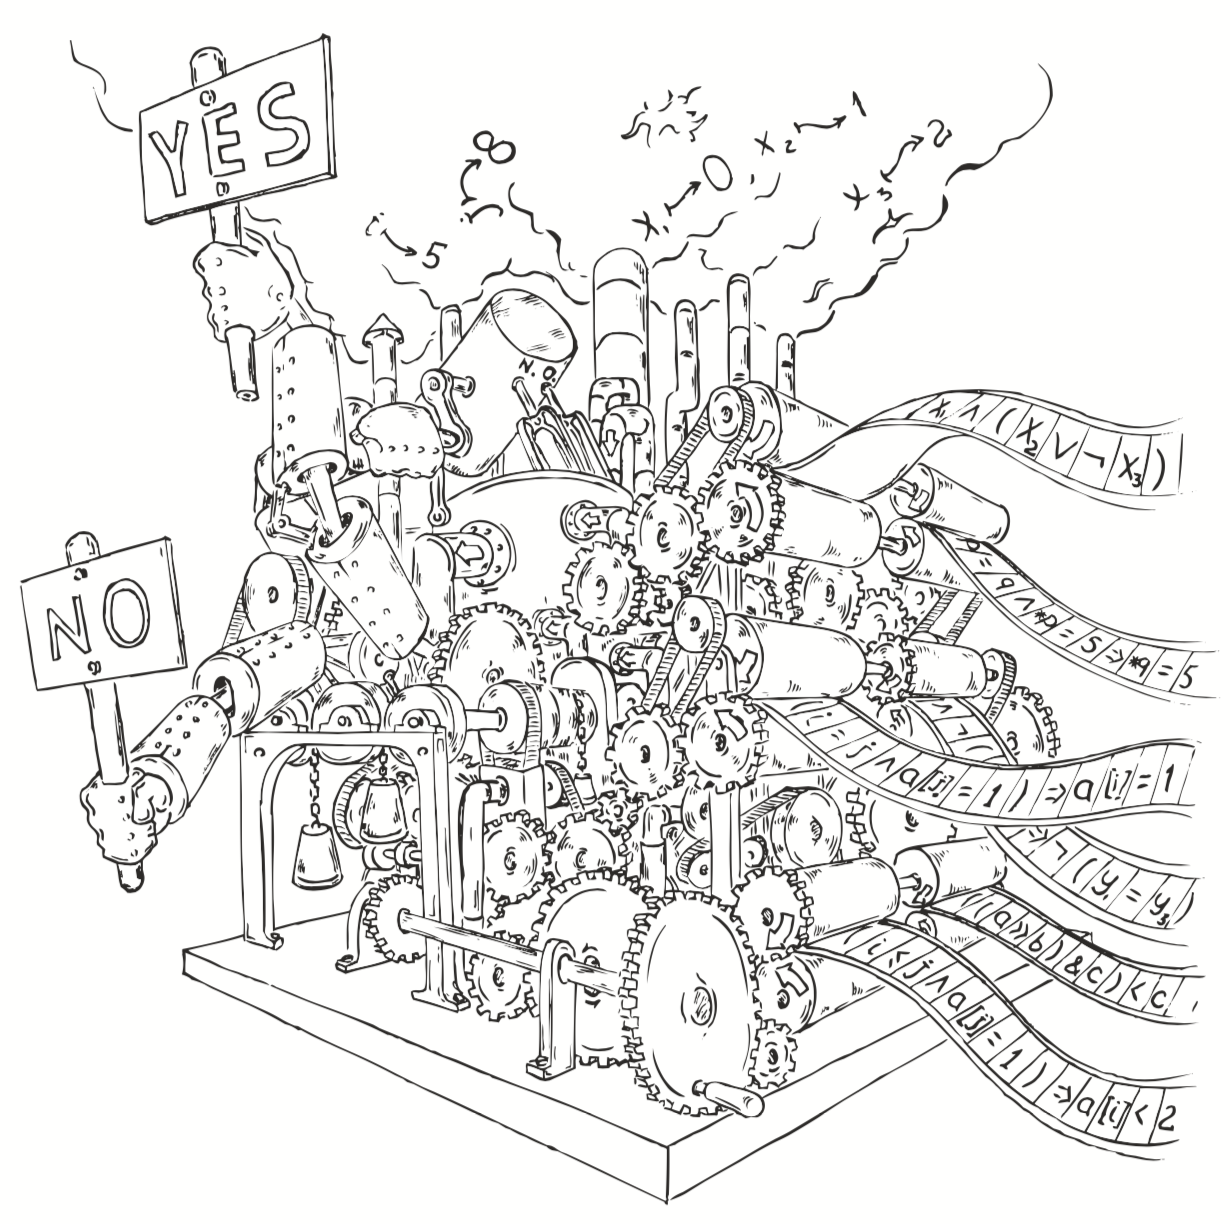
\includegraphics[scale=0.5]{../decision-procedure.png}
\end{frame}

\end{document}
